\documentclass[crop=false, class=book]{standalone}


\usepackage{graphicx}
\usepackage[italian]{varioref}
\usepackage{copyrightbox}

\begin{document}

	\section{Motion tracking}
	
		ARCore usa un processo chiamato \emph{Simultaneous localization and mapping (SLAM)} per determinare lo stato di un
		dispositivo che si trova all'interno di un ambiente sconosciuto. Questo stato è descritto dalla sua \textbf{posa} (posizione e orientazione) che viene stimata attraverso prestazioni di \emph{odometria} e \textbf{rilevazione di punti caratteristici}. Con odometria si intende l'uso di dati ricavati da sensori di movimento che permettono di valutare il cambiamento della posizione nel tempo. Nel caso degli smartphone viene utilizzato il sensore IMU che rileva misure inerziali (dati non visuali) come la velocita, accelerazione e posizione. La rilevazione di punti caratteristici è l'individuazione di immagini con caratteristiche differenti (dati visuali) che	consentono al dispositivo di calcolare la sua posizione relativa. Questi punti di riferimento insieme alle misurazioni ricavate dai sensori permettono di avere una buona stima della posa e di ricavare la rappresentazione di una mappa dell'ambiente circostante. Tuttavia, il movimento sequenziale stimato dallo SLAM include un certo margine di errore che si accumula nel tempo causando una notevole deviazione dai valori reali. Una soluzione che può essere adottata per risolvere questo problema consiste nel considerare come punto di riferimento un luogo visitato in precedenza di cui si sono memorizzate le sue caratteristiche \cite{mathworks2022slam}. Grazie alle informazioni di questo luogo è possibile minimizzare l'errore nella stima della posa.\\
		I contenuti virtuali possono essere renderizzati nella giusta prospettiva allineando la posa della telecamera virtuale con quella calcolata da ARCore. Il contenuto virtuale sembra reale perchè è sovrapposto all'immagine ottenuta dalla fotocamera del dispositivo.\\
		Nella figura \vref{fig: Motion Tracking} si può notare come la posizione dell'utente è tracciata in relazione ai punti caratteristici identificati nel divano reale.
		
		\begin{figure}
			\centering
			\copyrightbox[b]{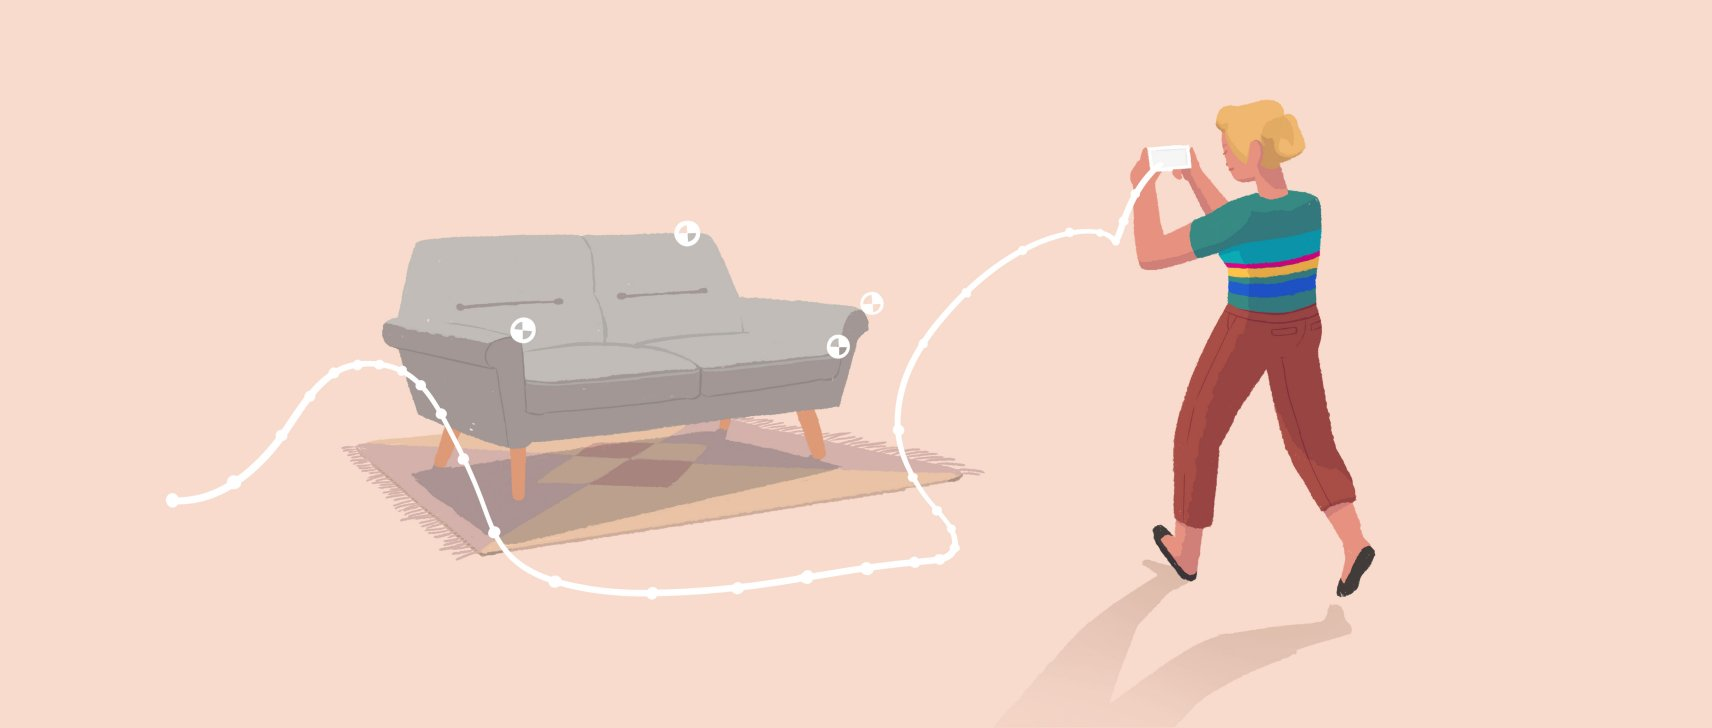
\includegraphics[width=0.8\textwidth]{./resources/images/MotionTracking/MotionTracking.jpg}}%
			{Fonte: \url{https://developers.google.com/ar/develop/fundamentals}}
			\caption{Motion Tracking.}
			\label{fig: Motion Tracking}
		\end{figure}
		
		\noindent
		Nella figura \vref{fig: Slam} sono rappresentati i moduli principali dello SLAM che si differenziano in quattro categorie \cite{andreasjakl2018slam}:
		
		\begin{itemize}
			\item \emph{Sensori}: nel caso degli smartphone fotocamera, sensore IMU (accelerometro, giroscopio). Potrebbero essere inclusi altri sensori per migliorare la precisione come GPS, sensori di luce, profondità.
			\item \emph{Front-end}: riceve i dati (visuali e non visuali) che permettono di ricavare una stima della posa. Dai dati \textit{visuali} identifica i punti caratteristici dai quali vengono estratti i \textit{descrittori di features}; mentre da quelli \textit{non visuali} ricava una stima precisa della posa correlando le caratteristiche spaziali di un frame con quelle osservate in sequenze di frame. I descrittori di features descrivono orientazione, scala, gravità, direzione e altri aspetti. Questo modulo include il riconoscimento dei luoghi già visitati se le stesse features vengono associate molte volte ai punti caratteristici.
			\item \emph{Back-end}: elabora l'output del front-end dal quale crea una rappresentazione 3d dell'ambiente sulla base di una pluralità memorizzata di mappe, descrittori di features e dalla stima della posa del dispositivo. Successivamente passa questa ricostruzione geometrica alla SLAM estimate.
			\item \emph{SLAM estimate}: calcola una posa localizzata cercando di ridurre al minimo le discrepanze tra i descrittori di features estratti e memorizzati nel tempo.
		\end{itemize}
	
		\begin{figure}
			\centering
			\copyrightbox[b]{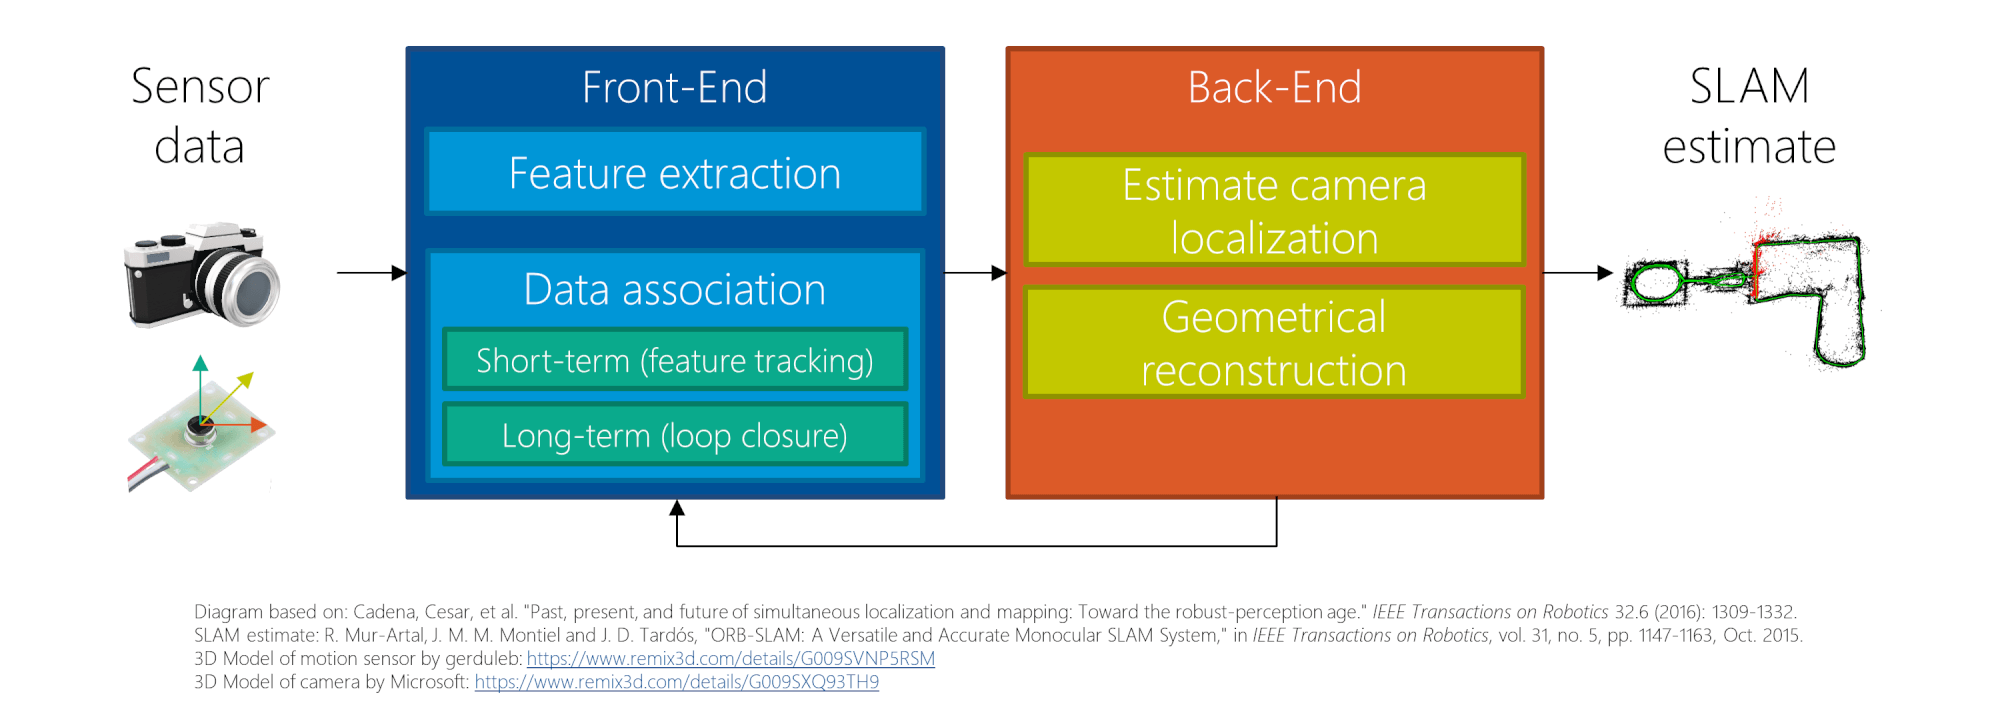
\includegraphics[width=1\textwidth]{./resources/images/MotionTracking/SLAM.png}}%
			{Fonte: \url{https://www.andreasjakl.com/basics-of-ar-slam-simultaneous-localization-and-mapping/}}
			\caption{Struttura dei moduli SLAM}
			\label{fig: Slam}
		\end{figure}
		
		\begin{figure}
			\centering
			\copyrightbox[b]{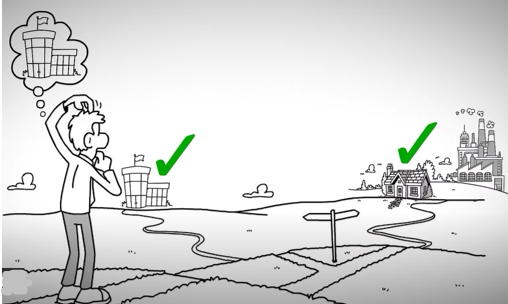
\includegraphics[width=0.6\textwidth]{./resources/images/MotionTracking/FeaturesPoints.png}}%
			{Fonte: \url{https://www.youtube.com/watch?v=UkIcupOTJrY&t=170s}}
			\caption{Punti caratteristici.}
			\label{fig: Punti caratteristici}
		\end{figure}
		
		\noindent
		Nell'esempio (a) in figura \vref{fig: Error Tracking} si può vedere come il margine di errore si accumula nel tempo portando ad una rappresentazione inconsistente della mappa dell'ambiente. In (b) si può notare un miglioramento della mappa allineando le varie scansioni in base ai vincoli imposti dalle pose relative. 
			
		\begin{figure}
			\centering
			\copyrightbox[b]{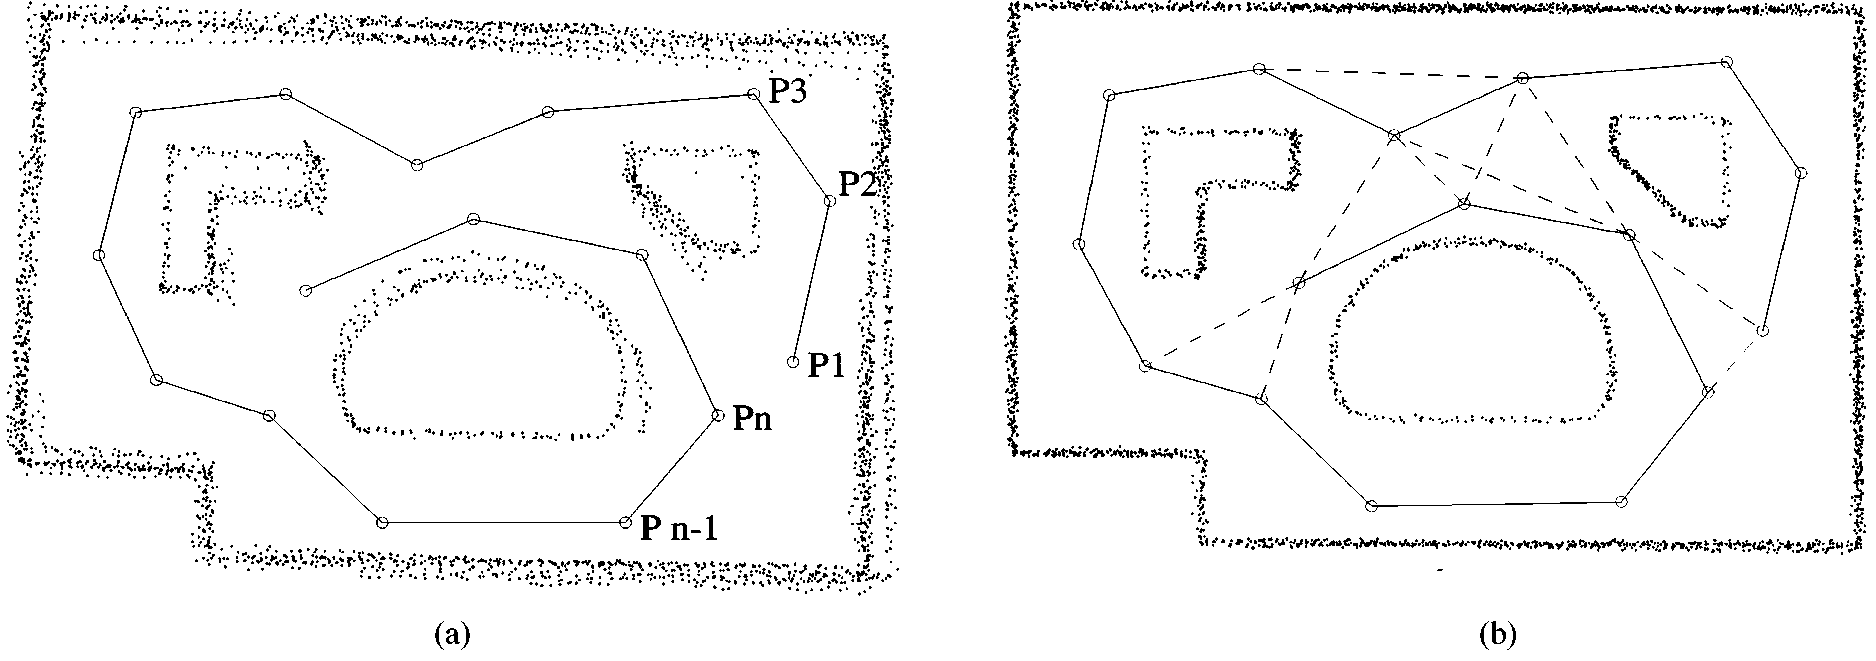
\includegraphics[width=0.8\textwidth]{./resources/images/MotionTracking/ErrorMap.png}}%
			{Fonte: \url{https://www.andreasjakl.com/basics-of-ar-slam-simultaneous-localization-and-mapping/}}
			\caption{Correzione degli errori da una mappa.}
			\label{fig: Error Tracking}
		\end{figure}
		
		\begin{flushleft}
			Per eseguire dei test sulle \textbf{performance} del Motion Tracking si devono tenere in considerazione alcuni aspetti:
		\end{flushleft}
		
		\begin{itemize}
			\item \emph{Angolazione}: l'abilità di rilevare punti caratteristici o superfici può dipendere dall'angolazione del dispositivo. Con alcuni angoli si potrebbero ottenere risultati migliori.
			\item \emph{Movimento}: questo test potrebbe essere iniziato con un movimento lento e con un aumento progressivo. A seguito di un movimento più rapido il dispositivo dovrebbe essere in grado di comprendere l'ambiente circostante e tracciare eventuali contenuti virtuali. Altri test possono essere effettuati con movimenti rapidi improvvisi e la copertura della fotocamera.
		\end{itemize}
		
		
		
		
		
	
\end{document}